\documentclass[journal]{IEEEtran}

\usepackage[T1]{fontenc}
\usepackage[utf8]{inputenc}
\usepackage{amsmath,amssymb,amsfonts}
\usepackage{graphicx}
\usepackage{booktabs}
\usepackage{algorithm}
\usepackage{algpseudocode}
\usepackage{cite}
\usepackage{url}
\usepackage{xcolor}
\usepackage[hidelinks]{hyperref}

\newtheorem{proposition}{Proposition}
\newtheorem{definition}{Definition}

\begin{document}

\title{SubSLD: Evidence-Paired Generation of Substation Single-Line Diagrams
from Volunteered Geographic Information}

\author{\IEEEauthorblockN{Ryuto~Shigenobu}
\IEEEauthorblockA{Department of Electrical, Electronic, and Computer Engineering,\\
University of Fukui, Fukui, Japan}}

\maketitle

\begin{abstract}
Public models of national transmission networks stop at the substation boundary:
what lies inside---busbars, bays, transformers, circuit counts---is proprietary
and therefore absent from open datasets. We present \emph{SubSLD}, a method that
reconstructs the internal composition of substations from volunteered geographic
information alone and renders it as an \emph{evidence-paired figure}: site
geometry over aerial imagery beside a machine-drawn single-line diagram. The
method is formulated as an evidence-closure operator whose output contains only
elements possessing an observational witness, so that soundness (``no
fabrication'') holds by construction; terminal binding is a lexicographic
maximisation over an ordered evidence vocabulary; circuit counts are produced by
a certified lower-bound estimator; and flow direction is a three-valued inference
that abstains explicitly rather than guessing. Applied to all of Japan, the
pipeline extracts 7{,}239 substation structures with 47{,}979 evidence-bound
terminals in about four seconds and renders paired figures for every site. We
report coverage rather than claim completeness: circuit evidence reaches
$68.2\,\%$ of 40{,}087 lines, busbar ways are mapped at only $14.2\,\%$ of sites
(from $53.3\,\%$ in Hokkaido to $5.1\,\%$ in Okinawa), and direction inference
abstains on $39.4\,\%$ of line groups. A photointerpretation review of fourteen
transmission substations lacking busbar ways finds that $64\,\%$ are mappable
omissions rather than physical absences, turning the measured gap into an
actionable contribution list for the source database. The extracted structure is
exported to CIM/CGMES---4{,}743 \texttt{BusbarSection}s and 8{,}475 \texttt{Bay}s
nationwide, with inferred elements flagged in their \texttt{description}---so the
result is consumable by standard power-system tooling. All artefacts are
regenerated by a single command and are published online.
\end{abstract}

\begin{IEEEkeywords}
Power system modelling, substations, single-line diagram, OpenStreetMap,
volunteered geographic information, open data, provenance.
\end{IEEEkeywords}

\section{Introduction}

\IEEEPARstart{O}{pen} models of electric power networks have advanced quickly:
continent-scale datasets derived from OpenStreetMap (OSM) now support
transmission-level studies, and several national models are published with
electrical parameters attached. These models share a boundary, however. They
describe how substations are \emph{connected}, but not what a substation
\emph{is}: the busbar sections it contains, how incoming lines attach to them,
how many circuits each line carries, and which voltage levels are joined by
transformers. That information sits in operator drawings and is not public.

The gap matters for two reasons. First, several analyses---bus-splitting,
breaker-level contingency screening, and hosting-capacity work at the bay
level---require internal structure that connectivity models cannot supply.
Second, and more subtly, the boundary hides the \emph{quality} of the open data:
when a model is drawn only as nodes and edges, one cannot see whether a
substation's representation rests on strong evidence or on a loose spatial
heuristic.

This paper takes the position that the interior of substations \emph{is} partly
observable in open data, provided the observation is treated with discipline.
Aerial imagery shows outdoor busbars and bay rows; OSM contains substation
polygons, in-yard ways tagged \texttt{line=busbar} or \texttt{line=bay}, and
transmission line ways carrying \texttt{circuits}, \texttt{cables} and
\texttt{wires} tags. What has been missing is not data but a method that (i)
asserts only what evidence supports, (ii) makes the strength of that evidence
visible in the output, and (iii) reports its own coverage as a result rather
than hiding it.

We propose \textbf{SubSLD} (evidence-paired substation single-line
diagramming). Its contributions are:

\begin{itemize}
\item \textbf{C1.} A formulation of substation structure extraction as an
      \emph{evidence-closure operator} (Section~\ref{sec:formulation}), with
      determinism, idempotence and soundness established by construction; the
      complement---completeness---is deliberately not claimed but measured.
\item \textbf{C2.} A \emph{certified lower-bound estimator} for circuit and
      conductor counts (Section~\ref{sec:estimation}), which formalises the rule
      ``never fill an untagged value by guessing'' as a guarantee that aggregates
      never overstate the physical asset.
\item \textbf{C3.} A \emph{three-valued direction inference} with explicit
      abstention (Section~\ref{sec:direction}), so that unresolved cases are
      rendered as unresolved instead of being silently resolved.
\item \textbf{C4.} A nationwide instantiation---7{,}239 substations, paired
      figures for every site, an in-browser viewer---together with a coverage
      evaluation and a photointerpretation study that converts the measured gaps
      into an OSM contribution list (Sections~\ref{sec:results}--\ref{sec:discussion}).
\item \textbf{C5.} A \emph{standards-conformant serialisation}
      (Section~\ref{sec:cim}): the node-breaker structure maps one-to-one onto
      CIM/CGMES classes, and the provenance of inferred elements survives the
      export, so downstream tools receive both the model and its caveats.
\end{itemize}

\section{Related Work}

OSM-derived power network models are well established at transmission level.
Continental extractions such as SciGRID and PyPSA-Eur build node--edge graphs and
attach electrical parameters by voltage-class heuristics; national efforts
follow the same pattern. All of them abstract a substation to a single node.
Where internal structure appears in open modelling, it is usually \emph{assumed}
(a single collector bus per voltage level) rather than extracted, because no
observational source was thought to exist.

Two adjacent literatures inform our approach. In data quality research for
volunteered geographic information, intrinsic indicators---completeness by
comparison against reference data, tag coverage, contributor density---are used
to characterise a dataset without ground truth; we adopt this stance and report
coverage as a primary result. In remote sensing, detection of transmission
infrastructure from aerial imagery (towers and conductors) is an active topic,
with public datasets such as TTPLA; we use imagery in a lighter role, as a human
verification and triage channel rather than as an automatic detector, and we
mark it as a distinct evidence class when it is used.

Our formulation is closest in spirit to provenance-carrying data integration:
each asserted element retains the witness that justified it, and the rendering
layer is required to display evidence strength. To our knowledge, no prior work
produces machine-generated single-line diagrams for a national fleet of
substations from open data with per-element provenance.

\section{Problem Setting}\label{sec:problem}

The input is a regional OSM extract: substation features (polygons or points),
line ways with geometry and tags, and in-yard ways. Coordinates are quantised to
approximately one metre,
\begin{equation}
q(p) = \bigl(\mathrm{round}(\phi,5),\ \mathrm{round}(\lambda,5)\bigr),
\end{equation}
which fuses duplicate registrations of the same facility, and the per-island
coordinate graph $G_I=(V_I,E_I)$ is formed over the nodes whose region belongs to
synchronous island $I$.

For a site $s$ we write $\mathrm{Poly}(s)$ for its footprint, $W_s$ for the
in-yard ways it contains, $W_\ell$ for the geometry of line $\ell$, and
$\mathrm{Terminals}(s)$ for the set of line ends bound to $s$. A voltage level is
denoted $v$ with nominal magnitude $kv_v$, and $L(s,v)$ is the set of lines bound
to that level. Table~\ref{tab:notation} summarises the notation.

\begin{table}[t]
\caption{Notation}
\label{tab:notation}
\centering
\begin{tabular}{ll}
\toprule
Symbol & Meaning \\
\midrule
$O$ & observation (polygons, ways, tags) \\
$S^{*}$ & extracted structure (node-breaker) \\
$\mathrm{Poly}(s)$ & site footprint of substation $s$ \\
$t\in\mathrm{Terminals}(s)$ & line end bound to $s$, carrying its evidence \\
$kv_v,\ L(s,v)$ & voltage level magnitude and its bound lines \\
$\hat{c}(w)$ & circuit-count estimate for way $w$ \\
$\mathrm{far}(g)$ & remote substations of line group $g$ \\
\bottomrule
\end{tabular}
\end{table}

\section{Formulation: Structure Extraction as Evidence Closure}
\label{sec:formulation}

\begin{definition}[Evidence closure]
Let $\mathrm{witnesses}(x,O)$ be the set of observations in $O$ that support the
existence of structural element $x$. The extraction operator is
\begin{equation}
F(O)\;=\;S^{*}\;=\;\bigl\{\,x \ \big|\ \mathrm{witnesses}(x,O)\neq\varnothing \,\bigr\},
\end{equation}
i.e.\ the largest structure all of whose elements are witnessed.
\end{definition}

This is the method proper; the algorithm below is one way to compute it.

\begin{proposition}[Properties of $F$]\label{prop:F}
\emph{(i) Determinism:} $F$ is a function---identical input yields byte-identical
structure (verified nationally by a regeneration test).
\emph{(ii) Idempotence:} re-application does not change the structure, so the
extraction may be embedded in a repeatedly executed regeneration pipeline.
\emph{(iii) Soundness:} every element of $S^{*}$ possesses a witness. This is
immediate from the construction and is the formal content of the ``no
fabrication'' rule.
\end{proposition}

Completeness---that every physically existing element appears in $S^{*}$---does
\emph{not} hold, because it is bounded by the coverage of $O$. We therefore do
not claim it; we measure it (Section~\ref{sec:results}).

\subsection{Terminal binding as lexicographic maximisation}

Line ends are attached to structure through an ordered evidence vocabulary,
\begin{equation}
\text{vertex} \;\succ\; \text{polygon} \;\succ\; \text{lead-in},
\end{equation}
with the predicates
\begin{align}
\mathrm{vertex}(t)&:\ \exists\,v\in W_\ell\cap W_s,\\
\mathrm{polygon}(t)&:\ p_{\mathrm{end}}(\ell)\in\mathrm{Poly}(s),\\
\mathrm{lead\text{-}in}(t)&:\ d\bigl(p_{\mathrm{end}}(\ell),\mathrm{Poly}(s)\bigr)\le\delta_{\mathrm{lead}},
\end{align}
where $\delta_{\mathrm{lead}}=0.6$\,km. The binding chosen for $t$ is
\begin{equation}
\mathrm{binding}(t)=\max\nolimits_{\succ}\{\,e \mid e \text{ witnesses } t\,\},
\end{equation}
and it is retained in the record, so that weak evidence can be drawn weakly
(lead-in bindings are rendered as dashed stubs).

\subsection{Consistency constraint}

Physical proximity is not electrical connection. Shared corridors and parallel
routes place lines of different classes within metres of one another, so the
closure is restricted by a voltage-consistency gate,
\begin{equation}
\mathrm{admit}(\ell,n) \iff
\mathrm{witnesses}\neq\varnothing \ \wedge\
\neg\bigl(|kv_\ell-kv_n| > 0.25\max(kv_n,1)\bigr).
\end{equation}
In our campaign this gate correctly rejected a $66$\,kV fragment touching a
$154$\,kV junction within $80$\,m; subsequent diagnosis showed the fragment
itself to be a cross-region registration artefact, i.e.\ the gate prevented an
error whose true cause lay elsewhere in the data.

\subsection{Algorithm}

\begin{algorithm}[t]
\caption{Structure extraction for one substation}
\label{alg:extract}
\begin{algorithmic}[1]
\Require site feature $s$, preprocessed ways $W$
\State $\mathrm{Poly}(s)\gets\mathrm{shape}(s)$; $V\gets\mathrm{vcls(tags)}\cup\mathrm{vcls(in\text{-}yard)}$
\ForAll{vertex-connected components of $W[\texttt{busbar}]$}
  \State emit \textsc{BusbarSection} (derive $kv$ from adjacency if untagged)
\EndFor
\ForAll{vertex-connected components of $W[\texttt{bay}]$}
  \State emit \textsc{Bay}, recording the busbars it touches
\EndFor
\ForAll{end points $p$ of line ways}
  \State $b\gets\max_\succ\{\text{vertex},\text{polygon},\text{lead-in}\}$
  \If{$b$ exists and $\mathrm{admit}$ holds}
     \State emit \textsc{Terminal}$(v,\ \mathrm{attach},\ b,\ \mathrm{par}=\hat{c}(w))$
  \EndIf
\EndFor
\State emit \textsc{Transformer} for adjacent voltage-class pairs (structural)
\State \textbf{if} a level has $\ge 2$ strongly-bound terminals and no busbar way
       \textbf{then} emit an \emph{inferred} busbar (marked)
\Ensure $S^{*}$ with a witness on every element
\end{algorithmic}
\end{algorithm}

Algorithm~\ref{alg:extract} realises $F$. The final step deserves comment: in
gas-insulated and indoor substations a busbar is not a visible way and can never
be observed, yet its existence is electrically necessary when two or more lines
bind strongly to the same level. We therefore emit an \emph{inferred} busbar,
recorded with \texttt{source = inferred-topology} and rendered dashed. This
asserts existence only---no geometry, no terminal re-binding---so soundness in
the sense of Proposition~\ref{prop:F} is preserved with the caveat made visible.

\begin{figure*}[t]
\centering
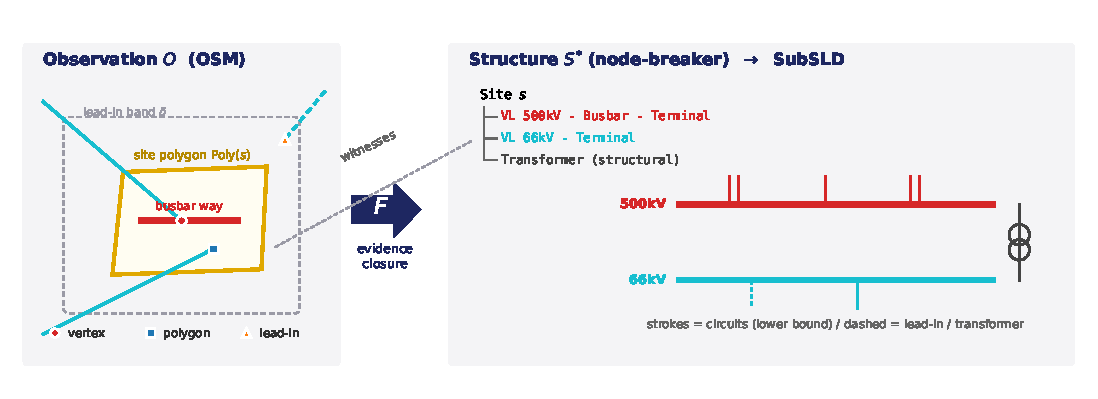
\includegraphics[width=\textwidth]{figs/fig_concept.pdf}
\caption{The SubSLD method. Observation $O$ (site polygon, in-yard busbar way,
line ends with their binding evidence, lead-in band $\delta$) is mapped by the
evidence closure $F$ to a node-breaker structure $S^{*}$, which is rendered as
the paired figure. Every drawn element retains the witness that justified it.}
\label{fig:concept}
\end{figure*}

\section{Estimation of Circuit and Conductor Counts}\label{sec:estimation}

OSM line ways carry \texttt{circuits}, \texttt{cables} and \texttt{wires} tags
irregularly. Rather than imputing missing values, we define
\begin{equation}
\hat{c}(w)=
\begin{cases}
c_{\mathrm{tag}}(w), & \text{if \texttt{circuits} is present},\\[2pt]
\lfloor n_{\mathrm{cables}}(w)/3\rfloor, & \text{else if \texttt{cables} is present},\\[2pt]
1, & \text{otherwise},
\end{cases}
\end{equation}
and aggregate per site and voltage level while keeping evidence and estimate
apart,
\begin{equation}
c_{\mathrm{est}}(s,v)=\!\!\sum_{w\in L(s,v)}\!\!\hat{c}(w),
\qquad
c_{\mathrm{sum}}(s,v)=\!\!\sum_{w:\,\mathrm{evidence}}\!\!\hat{c}(w).
\end{equation}

\begin{proposition}[Lower bound]\label{prop:lb}
Under (A1) a present \texttt{circuits} tag is correct and (A2) a three-phase
circuit uses at least three conductors,
\begin{equation}
c_{\mathrm{sum}}(s,v)\ \le\ c_{\mathrm{est}}(s,v)\ \le\ c_{\mathrm{true}}(s,v).
\end{equation}
\end{proposition}

\begin{IEEEproof}
Termwise, $\hat{c}(w)\le c_{\mathrm{true}}(w)$: with a tag this is (A1); with
only \texttt{cables} the floor of $n_{\mathrm{cables}}/3$ under-counts by (A2);
and an existing way carries at least one circuit. Summation preserves the
inequality, and $c_{\mathrm{sum}}$ omits non-negative terms of $c_{\mathrm{est}}$.
\end{IEEEproof}

The practical consequence is that a SubSLD figure states ``at least this many
circuits exist''. When such counts are used downstream---for corridor capacity
proxies, for instance---the error is on the conservative side. Conductor bundles
(\texttt{wires}) are treated identically.

\section{Three-Valued Direction Inference}\label{sec:direction}

Whether a line feeds a substation or is fed by it is not tagged. We order
substations by their highest voltage level and infer
\begin{equation}
\hat{d}:\ G \longrightarrow \{\,\mathrm{in},\ \mathrm{out},\ \bot\,\}
\end{equation}
for each line group $g$ with remote set $\mathrm{far}(g)$:
\begin{align}
\hat{d}(g)=\mathrm{in} &\iff
\exists s'\!\in\!\mathrm{far}(g):\ kv_{\max}(s') > kv_v
\ \ \vee\ \ kv_v = kv_{\mathrm{top}}(s),\\
\hat{d}(g)=\bot &\iff \mathrm{far}(g)=\varnothing,\\
\hat{d}(g)=\mathrm{out} &\quad\text{otherwise}.
\end{align}
$\mathrm{far}(g)$ is resolved from derived site-to-site connections, falling back
to line names of the form ``$A$--$B$ line'' when connections are missing. The
third value is the point: when the remote end is unknown---overwhelmingly because
the remote substation itself is absent from OSM---the method abstains and the
figure renders the stub in grey. The abstention rate is reported as an evaluation
metric, not suppressed.

\section{Implementation and Results}\label{sec:results}

The pipeline has three stages: extraction (Algorithm~\ref{alg:extract}),
property aggregation (Section~\ref{sec:estimation}), and rendering. All stages
are deterministic and idempotent and are embedded in the project's single
regeneration command, so the entire layer is reproducible in one pass.

\begin{table}[t]
\caption{Nationwide extraction (all of Japan, 10 regions)}
\label{tab:scale}
\centering
\begin{tabular}{lr}
\toprule
Quantity & Value \\
\midrule
Substation structures extracted & 7{,}239 \\
Evidence-bound terminals & 47{,}979 \\
Busbar sections (observed) & 2{,}559 \\
Busbar sections (inferred, marked) & 2{,}669 \\
Bays & 8{,}753 \\
Transformers (structural) & 2{,}590 \\
Site-to-site connections derived & 11{,}586 \\
Extraction time (whole country) & $\approx 4$\,s \\
Paired-figure rendering & 1--6\,s per site \\
\bottomrule
\end{tabular}
\end{table}

Table~\ref{tab:scale} summarises the national instantiation. Rendering the whole
country produced paired figures for every site; on a 160-thread server with ten
regional workers the full sweep completed in about one hour with zero failures.

\begin{figure*}[t]
\centering
\begin{minipage}[t]{0.40\textwidth}
\centering
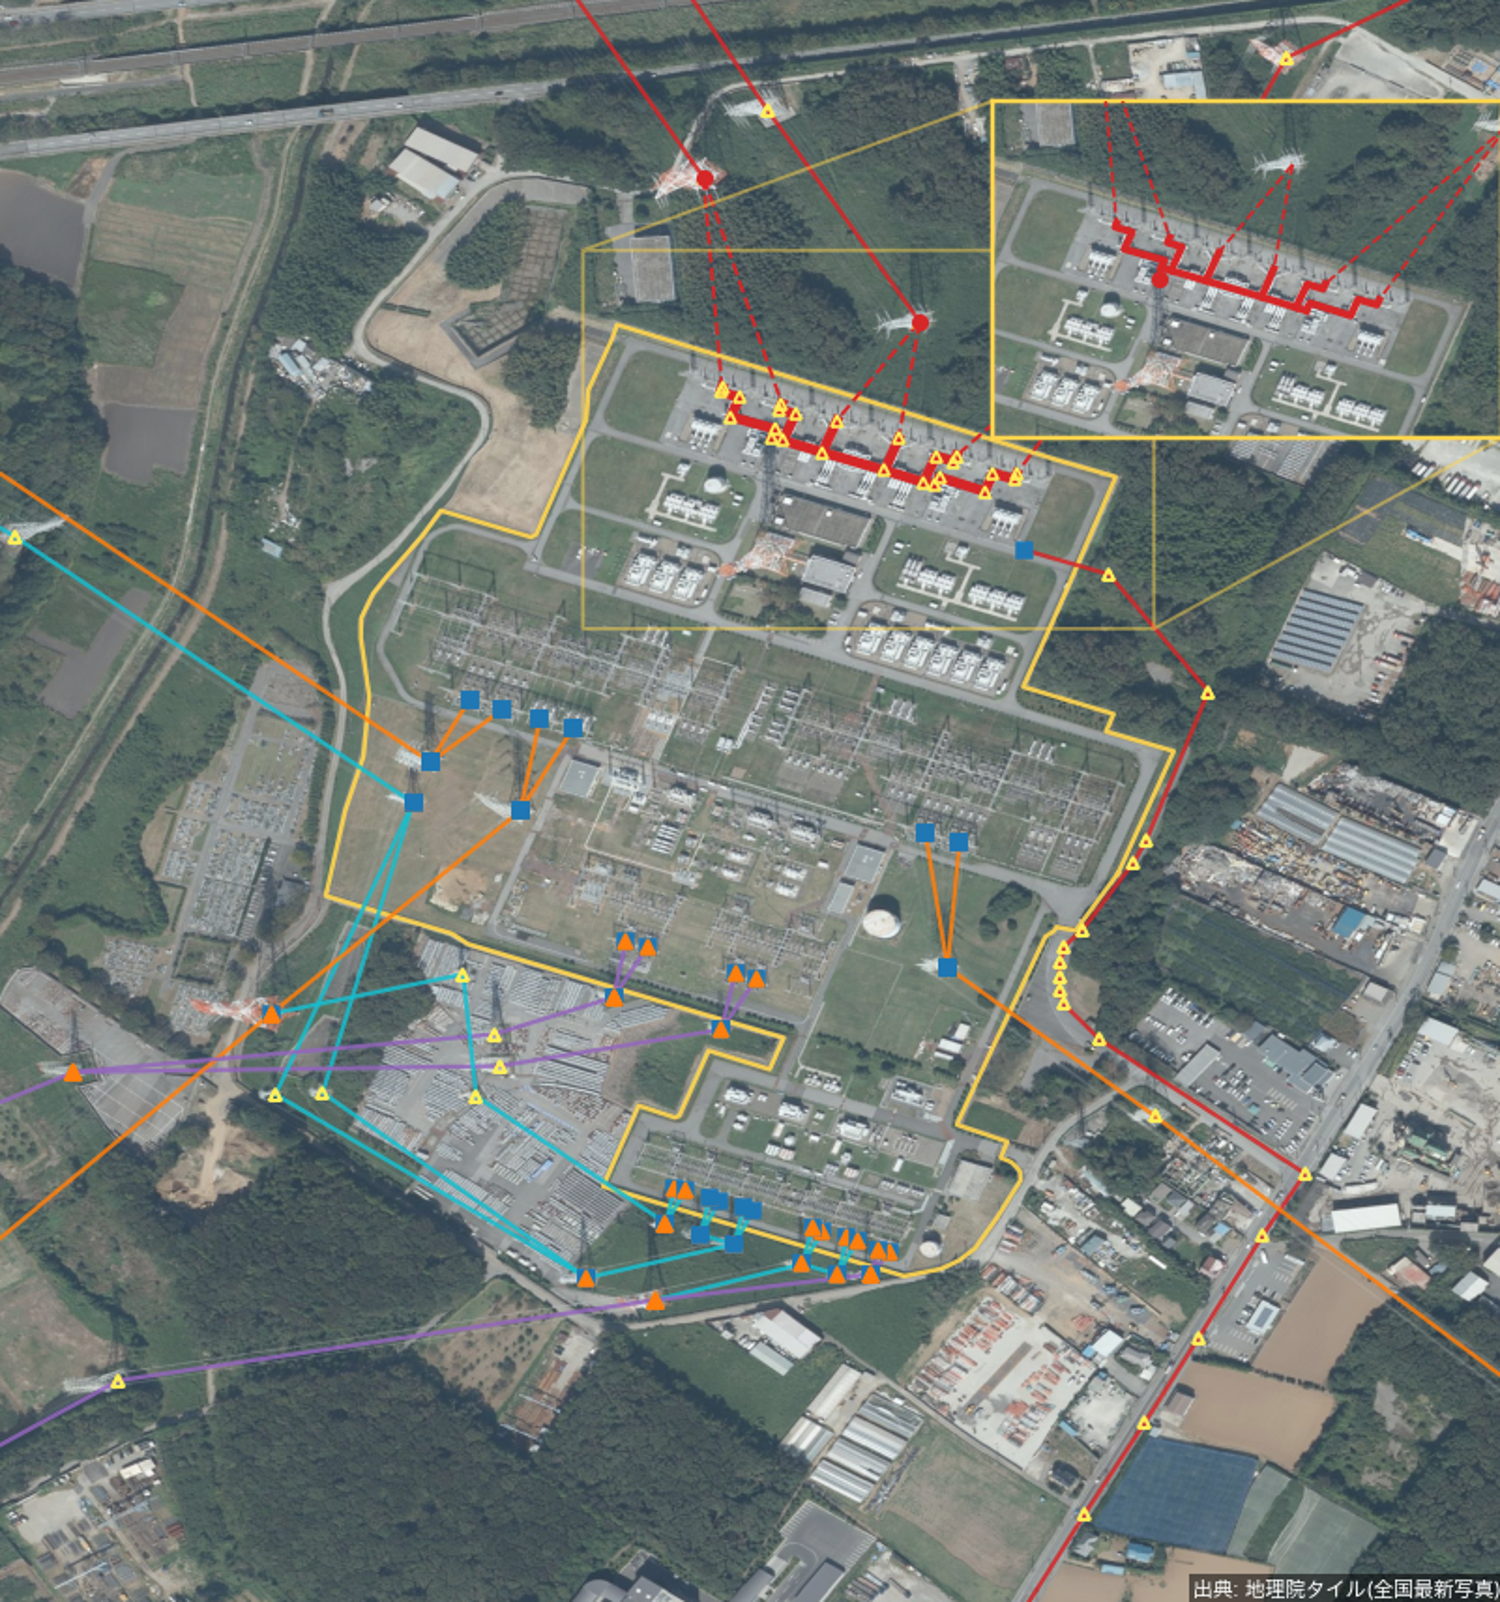
\includegraphics[width=\textwidth]{figs/fig_pair_geo.png}\\[2pt]
{\footnotesize (a) GeoPane}
\end{minipage}\hfill
\begin{minipage}[t]{0.57\textwidth}
\centering
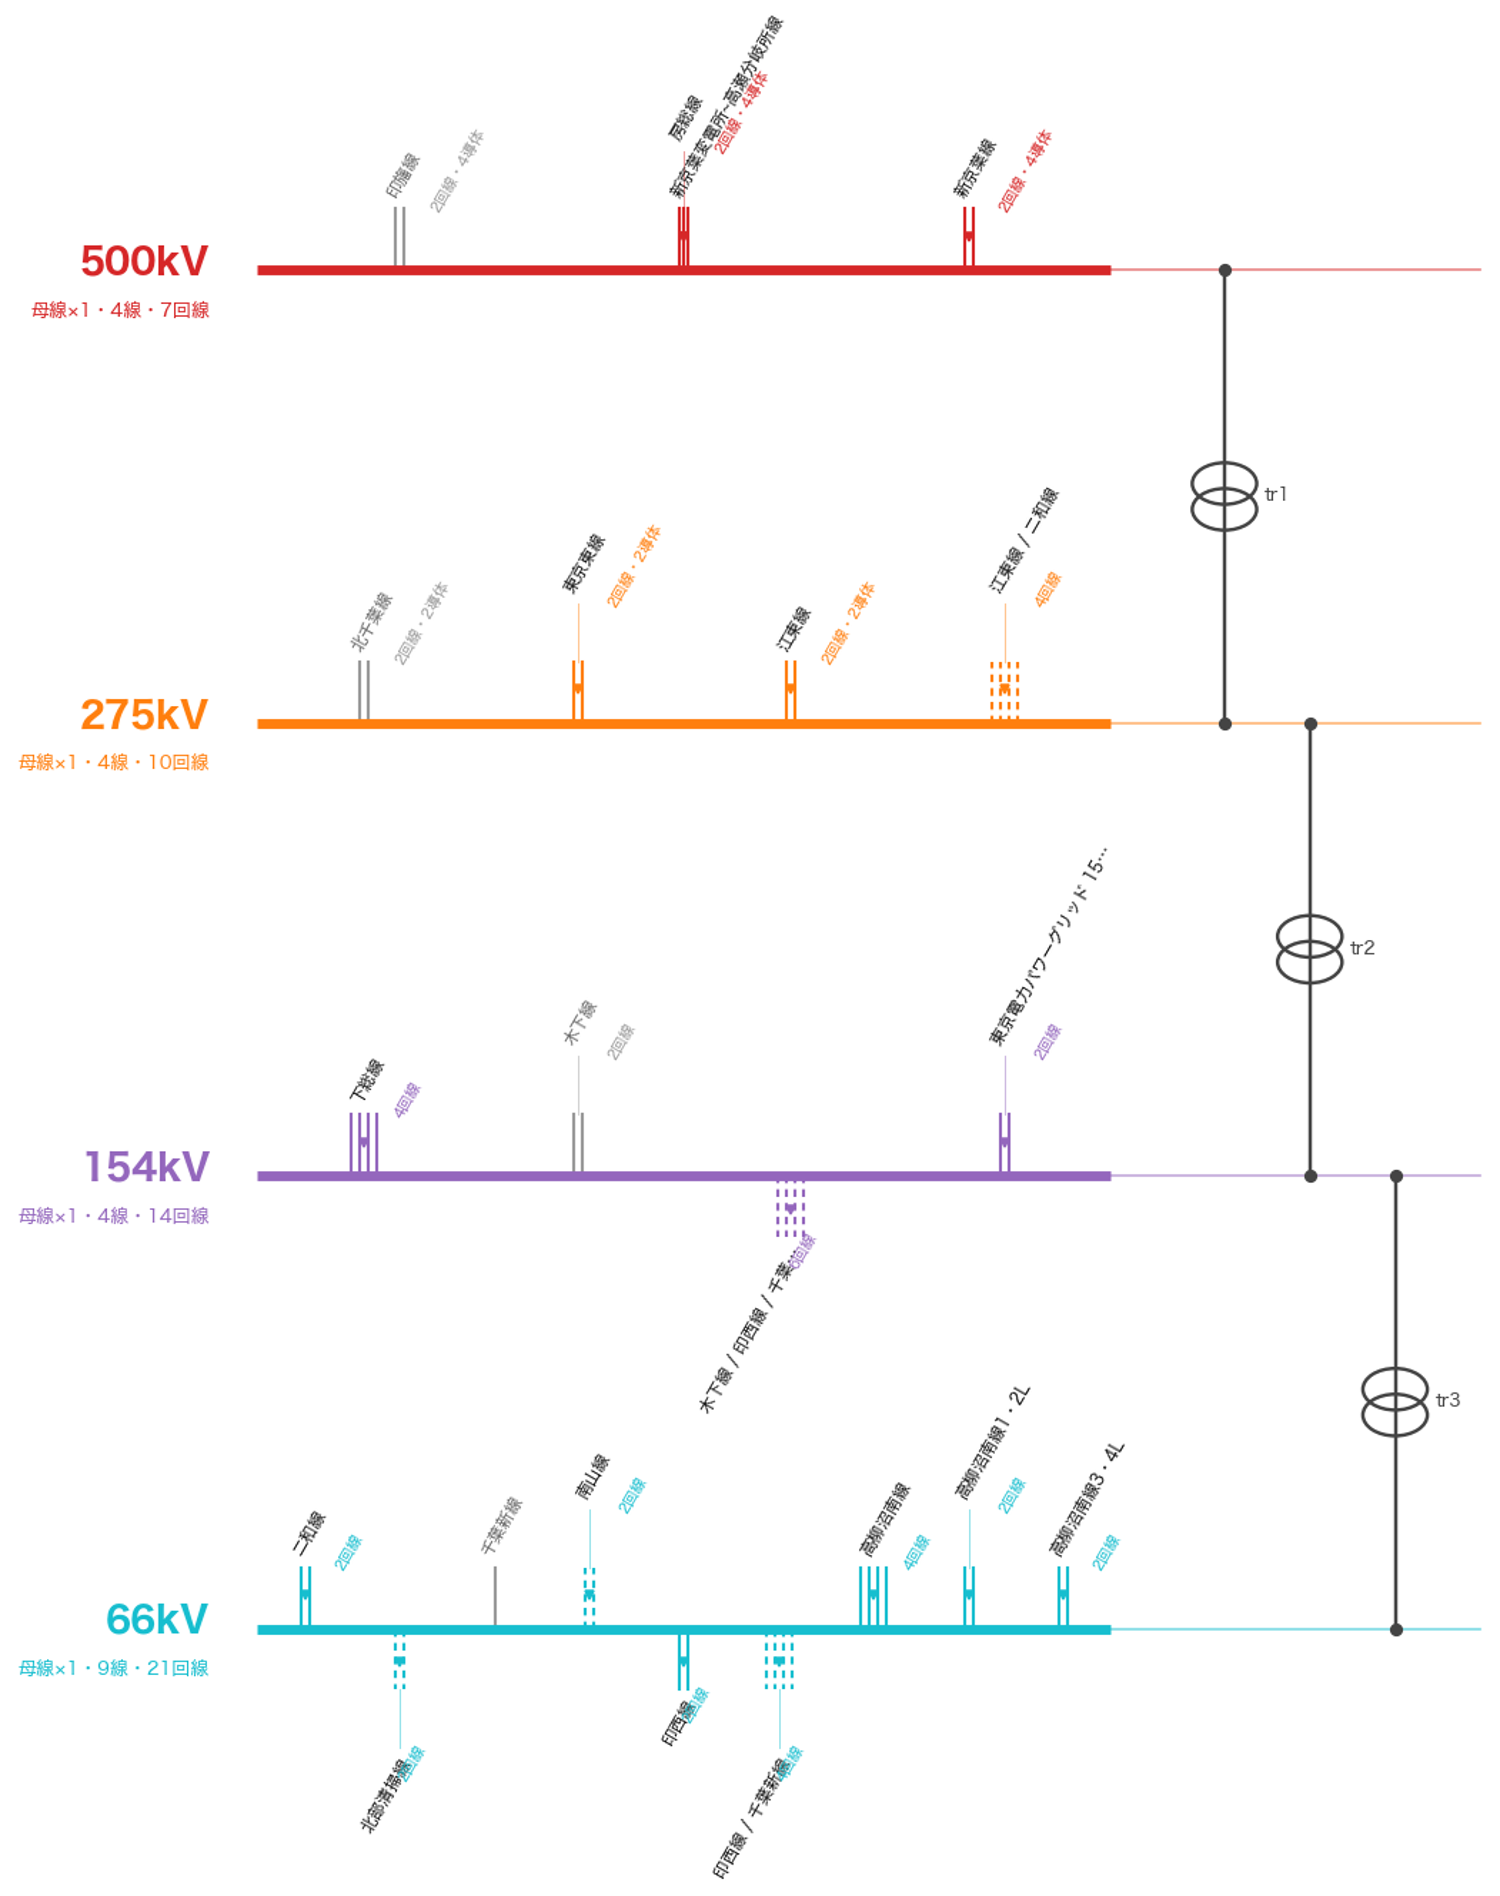
\includegraphics[width=\textwidth]{figs/fig_pair_sld.png}\\[2pt]
{\footnotesize (b) SLDPane}
\end{minipage}
\caption{Evidence-paired figure for a $500/275/154/66$\,kV substation
(Shin-Keiyo). (a) Site outline, in-yard busbar geometry, real line geometry by
voltage class, and binding markers over aerial imagery. (b) Machine-drawn
single-line diagram: busbar sections, one stroke per circuit, dashed stubs for
lead-in evidence, grey for abstained direction, transformers between levels.
Imagery: GSI seamless photo tiles.}
\label{fig:pair}
\end{figure*}

Fig.~\ref{fig:pair} shows a representative output. The left pane is the audit
surface---one can see which line the diagram is talking about and how strongly it
is attached---while the right pane is the electrical reading of the same
evidence.

\subsection{Coverage}

\begin{figure*}[t]
\centering
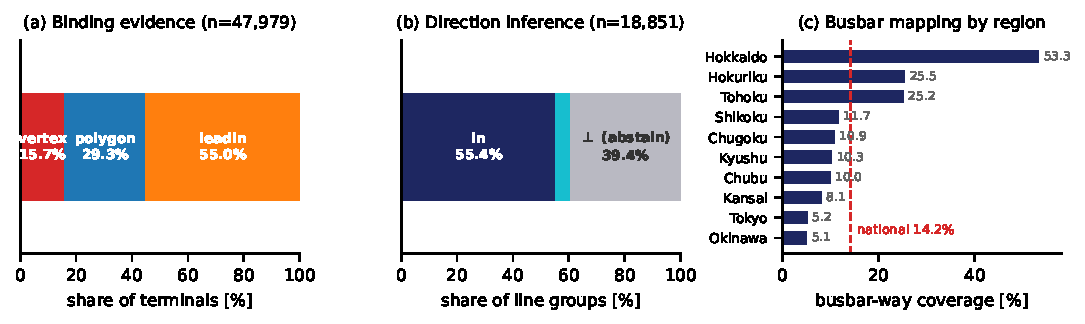
\includegraphics[width=\textwidth]{figs/fig_coverage.pdf}
\caption{Coverage measured on the national extraction. (a) Distribution of
terminal binding evidence. (b) Outcome of direction inference, including
explicit abstention. (c) Busbar-way mapping rate by region, against the national
mean.}
\label{fig:coverage}
\end{figure*}

Fig.~\ref{fig:coverage} reports what the method could and could not observe.
Circuit evidence (a \texttt{circuits} or \texttt{cables} tag) exists for
$68.2\,\%$ of 40{,}087 lines; conductor-bundle tags for only $12.7\,\%$.
Terminal binding is dominated by the weakest class: $55.0\,\%$ lead-in,
$29.3\,\%$ polygon, $15.7\,\%$ vertex. Direction inference returns
$\mathrm{in}$ for $55.4\,\%$ and $\mathrm{out}$ for $5.2\,\%$ of 18{,}851 line
groups and abstains on $39.4\,\%$.

The sharpest limitation is busbar mapping: only $14.2\,\%$ of sites have a busbar
way, with a strong regional gradient---$53.3\,\%$ in Hokkaido against $5.1\,\%$
in Okinawa and $5.2\,\%$ in Tokyo (Fig.~\ref{fig:coverage}(c)). Point-geometry
sites, which cannot host in-yard ways at all, are mapped at $3.2\,\%$.

\subsection{Photointerpretation of the busbar gap}

Is the gap a mapping omission or a physical absence? We reviewed fourteen
transmission substations that lack busbar ways, using their own SubSLD GeoPanes
over aerial imagery. Nine ($64\,\%$) show outdoor air-insulated busbars and bay
rows plainly visible from above---mappable omissions. One has in-yard ways and
vertex-shared terminals but no \texttt{line=busbar} tag, i.e.\ a tagging omission
repairable without new geometry. The remaining five are gas-insulated or indoor
installations in which no busbar exists as a visible line and for which the
inferred-busbar mechanism is the appropriate answer.

This diagnosis converts a coverage statistic into work: the nine mappable sites,
together with a transmission line found by satellite review but absent from OSM,
were published as a contribution list with per-site edit links.

\section{Standards-Conformant Export}\label{sec:cim}

A method that produces structure only for its own renderer has limited reach.
The data model of Section~\ref{sec:formulation} was therefore defined against
CIM from the outset, and each class maps one-to-one onto its CGMES counterpart
(Table~\ref{tab:cim}). Exporting is consequently a direct serialisation rather
than a translation.

\begin{table}[t]
\caption{Mapping of the extracted structure onto CIM/CGMES, with national counts}
\label{tab:cim}
\centering
\begin{tabular}{llr}
\toprule
SubSLD element & CIM/CGMES class & Exported \\
\midrule
SubstationSite   & \texttt{cim:Substation}      & 7{,}240 \\
VoltageLevel     & \texttt{cim:VoltageLevel}    & per site, per class \\
BusbarSection    & \texttt{cim:BusbarSection}   & 4{,}743 \\
\quad of which inferred & (flagged, see text)   & 2{,}289 \\
Bay              & \texttt{cim:Bay}             & 8{,}475 \\
TransformerSpec  & \texttt{cim:PowerTransformer} & 2{,}590 \\
Terminal         & \texttt{cim:Terminal}        & with \texttt{ConnectivityNode} \\
\bottomrule
\end{tabular}
\end{table}

Two points of discipline carry over into the export. First, a bay touching two
busbar sections of the same voltage level is a coupler candidate, and this is
disclosed in the object name rather than asserted as a breaker, because no
switch was observed. Second---and more important for a consumer of the
file---\emph{inferred busbars remain marked}. CGMES~2.4 has no attribute for
``estimated'', so the provenance is written into
\texttt{IdentifiedObject.description}:

\begin{quote}\footnotesize\ttfamily
inferred-topology (SubSLD): no busbar way in OSM;\\
existence derived from strongly-bound terminals
\end{quote}

A tool that ignores the field still receives a valid, solvable topology; a tool
or an analyst that reads it can separate the $2{,}454$ observed busbars from the
$2{,}289$ inferred ones. The same principle governs transformer ratings
elsewhere in the project: \texttt{ratedS} is written only where a nameplate
source exists, never synthesised to fill the attribute.

The export runs as one stage of the regeneration pipeline over all ten regions,
producing CGMES EQ and GL profiles; a Level-2 export (EQ/TP/SSH/SV) exists in
the same project and has been round-tripped through an independent CIM importer
to confirm the resulting cases still solve. The node-breaker layer introduced
here rides on that established path.

\section{Discussion}\label{sec:discussion}

\emph{Showing the gap is part of the result.} A model that silently completes
missing structure produces a figure that looks finished and is therefore
unauditable. SubSLD instead propagates evidence strength into the rendering:
dashed stubs for lead-in bindings, grey for abstained direction, dashed busbars
for inference. A reader can see, per element, how much to trust the drawing---and
the same visual grammar identifies where the open database should be improved.

\emph{Limits.} The lead-in band admits nearby passing lines as weak evidence;
this is visible but not eliminated. Direction inference is a voltage-hierarchy
heuristic, not a power-flow result, and is labelled as inference throughout.
Conductor-count coverage is low enough that bundle information should be treated
as sparse annotation rather than a field. Finally, all coverage figures are
snapshots of a living database.

\emph{Outlook.} Three directions follow naturally. Automatic detection of towers
and busbars from imagery would raise the evidence base without human review.
The contribution list closes a loop in which the model improves its own source.
And a bay-level structure with inferred busbars is the precondition for
breaker-level analyses on an open national model.

\section{Conclusion}

We have shown that the internal composition of substations can be reconstructed
nationwide from volunteered geographic information, provided extraction is
formulated so that soundness holds by construction, estimation is certified as a
lower bound, and inference is allowed to abstain. Applied to Japan, SubSLD
produced structures for 7{,}239 substations with 47{,}979 evidence-bound
terminals and an evidence-paired figure for every site, alongside an honest
account of what open data does not yet contain. The measured gaps are not a
postscript to the result---they are the part of it that tells the community what
to map next.

\section*{Data and Code Availability}

The method, generators, viewer and datasets are part of the All-Japan-Grid
project (\url{https://github.com/lutelute/All-Japan-Grid}), released as
\texttt{v1.8.0}; CGMES EQ/GL exports including the node-breaker layer are
regenerated by \texttt{scripts/export\_cim.py}. The nationwide viewer is at
\url{https://lutelute.github.io/All-Japan-Grid/subsld.html}. Aerial imagery is
from the Geospatial Information Authority of Japan; base map data
\copyright\ OpenStreetMap contributors (ODbL).

\section*{Acknowledgment}

The author thanks the OpenStreetMap contributors whose mapping makes this work
possible.

\end{document}
